%%%%%%%%%%%%%%%%%%%%%%%%%%%%%%%%%%%%%%%%%%%%%%%%%%%%%%%%%%%%%%%%%%%%%%%%%%%%%%%%%%%%%%%%%%%
%                               Evaluation - 16pp
%%%%%%%%%%%%%%%%%%%%%%%%%%%%%%%%%%%%%%%%%%%%%%%%%%%%%%%%%%%%%%%%%%%%%%%%%%%%%%%%%%%%%%%%%%%
\chapter{Evaluation}
\label{sec:evaluation}

\section*{Summary}
%To evaluate our approach we plan to run several experimental tests within a group of, at least, ten subjects. 
%With these experiments we want to obtain statistical measures about our approach and be able to conclude 
%on which combinations of feedback could have better performance in guiding a patient.

%We will be using two different experiments in order to achieve comparable results. 
%The first experiment will consist of a \ac{PT} and a test subject. 
%The \ac{PT} will demonstrate a given exercise to the test subject and then evaluate their execution without giving any kind of feedback. 

%The second experiment will involve guiding a test subject through the same exercise as the first experiment, 
%using different combinations of visual, audio and haptic feedback.
%The resulting performance will be analyzed and several data gathered. 
%We will take into account the following metrics, (a) the trajectory error between the Exercise Model and 
%the patient's actual execution, (b) the time it takes for the patient to finish the exercise 
%and (c) the time it takes for the patient to recover to the correct position if mistaken.

%We will start by using a unimodal approach, to obtain measurements using only one of the 
%available feedback modes each time. After the unimodal experiments, we will begin the multimodal 
%approach experiments by combining the available feedback and repeat the same measurements previously done.

%Even though our main focus is to provide concurrent feedback (during the execution), its frequency will be altered in order to evaluate the patient response. Therefore, further in the end, we will provide only terminal feedback (without guiding cues during the execution) to analyze if the patient successfully learned the movement.

To evaluate SleeveAR, we intended to observe how well a subject recreates simple arm movements just by following the feedback at his disposal. 
Since tests involve executing simple arm movements, five different exercises were created for this evaluation. These exercises were simultaneously recorded both by video and by the SleeveAR's recording features. This way, we guarantee the same movement is being stored in video and in our system.

This chapter presents a detailed description of the experimental tests. It addresses the experimental methodology employed for testing our prototype with test subjects, the category of performed tests, the measurement metrics, and the characteristics of the collected sensor information. It also presents the experimental results and their critical analysis. All the results will be discussed in order to achieve a better understanding about our prototype functionality and performance.
Finally, the chapter reports some of the most important critics elaborated by a professional physical therapist after using our system.

\section{Methodology} \label{evaluation-methodology}

\begin{table}
\centering
\begin{tabular}{lll}
\hline
\multicolumn{1}{|l|}{\#}& \multicolumn{1}{l|}{Stage}         & \multicolumn{1}{l|}{Time}       \\ \hline
\multicolumn{1}{|l|}{1} & \multicolumn{1}{l|}{Introduction}  & \multicolumn{1}{l|}{2 minutes}  \\ \hline
\multicolumn{1}{|l|}{2} & \multicolumn{1}{l|}{SleeveAR}      & \multicolumn{1}{l|}{15 minutes} \\ \hline
\multicolumn{1}{|l|}{3} & \multicolumn{1}{l|}{Video}         & \multicolumn{1}{l|}{10 minutes} \\ \hline
\multicolumn{1}{|l|}{4} & \multicolumn{1}{l|}{Questionnaire} & \multicolumn{1}{l|}{3 minutes}  \\ \hline
\end{tabular}
\caption{SleeveAR evaluation stages}
\label{table:teststages}
\end{table}

%\begin{itemize}
%\item divided by 3 main parts
%\item executing movements following video instructions
%\item executing movements following SleeveAR
%\item answering a small form at the end
%\end{itemize}

This section describes the experimental methodologies for testing our prototype. Each participant followed this methodology in a similar way.

The average time spent with each participant was approximately thirty minutes. As we can observe in Table~\ref{table:teststages}, the test was composed of four stages:

\begin{enumerate}
\item \textbf{Introduction}

Before the actual test, participants received a brief explanation concerning the main goal of our thesis. They were also made aware of what would the full experimental test consist of.

\item \textbf{SleeveAR}

The participant executes the exercises, as described in Section~\ref{evaluation-tasks}, while following our prototype real-time feedback.

\item \textbf{Video}

For each of the five exercises selected for this evaluation, the participant  watches a video of its execution at least two times. Then, while following the video playing, the participant executes the same movement based on the video observation.

\item \textbf{Questionnaire}

Finally, a small questionnaire should be filled by the participant. This questionnaire includes questions concerning stage 2 and 3, while also providing us some information about the user's profile.

\end{enumerate}

In order to gather data for further result analysis, each execution of an exercise generated a Log with all the necessary information about the participant's movement.

Even though we are presenting this ordering for the four stages, half of the participants started by doing the third stage before the second, for the purpose of obtaining a more balanced sample of results.

\section{Performed Tasks} \label{evaluation-tasks}


Participants were asked to execute five different exercises which consisted of rather simple combinations of possible anatomic arm movements, described previously.
Each exercise consisted of different movement combinations which can be seen in Table~\ref{table:exercises}.
These same five exercises were executed for both the above mentioned second and third stages.
To store the original exercise we first had to capture it, hence, each exercise was simultaneously recorded with a video camera and with motion tracking devices. Under these circumstances, we made sure that the content being stored in video format directly represented the data being stored on SleeveAR's prototype.

While in the SleeveAR phase, the users would first be presented with a small tutorial which introduced interactively each of the feedback components individually. 
More specifically, the forearm feedback, followed by the upper arm feedback and finishing with its combination.
After the tutorial, both the SleeveAR and Video phases had the same methodology. 
The user had three attempts for each exercise, being the first two more aimed at practicing the exercise.

% Please add the following required packages to your document preamble:
% \usepackage{graphicx}
\begin{table}[!t]
\centering
\scalebox{0.8}{
\begin{tabular}{|c|c|c|c|}
\hline
\textbf{Exercises} & \textbf{Abduction/Adduction} & \textbf{Elevation/Depression} & \textbf{Flexion/Extension} \\ \hline
1 & \ding{51} &  &  \\ \hline
2 & \ding{51} & \ding{51} &  \\ \hline
3 & \ding{51} &  & \ding{51} \\ \hline
4 &  & \ding{51} &  \\ \hline
5 & \ding{51} & \ding{51} & \ding{51} \\ \hline
\end{tabular}
}
\caption{Arm movements in exercises.}
\label{table:exercises}
\end{table}


\section{Participants} 


The participants in this trial were invited randomly and were mainly students attending our educational
institution. Thereby, the set of test users was comprised of 18 participants, consisted of 14 males and 4 females,
and all with a college degree. In regard to their age, we had an average age of approximately 26 years old. 
All participants declared not having any physical impairment at the moment of the tests. 
The test users profile gathered from the questionnaire is available in Appendix~\ref{appendix_questionnaire}.
It should be noted one of our participants was a professional physical therapist. 
In Section~\ref{sec:pt} the full interaction with this participant is described.


\section{Results and Discussion}
\label{sec:results}

In this section, we present an analysis of the data obtain during the evaluation sessions.
The data gathered consists of user preferences and task performance.
The main objective was to address the correctness of the executed exercises. 
Experiments with test subjects were performed for a baseline scenario, consisting of exercise execution through video observation, and for a patient assisted scenario consisting of real-time feedback provided the proposed prototype. 
Furthermore, this evaluation provides a formal study of our feedback techniques.
Therefore, the analysis of the results is divided into a {\it User Preferences Overview} and {\it Task Performance Overview}. 
A discussion of the final results is also provided along this section.

\subsection{User Preferences Overview}

\begin{table}[!t]
\centering
\scalebox{0.8}{
\begin{tabular}{l|c|c|}
\cline{2-3}
\textbf{}                                                          & \multicolumn{2}{c|}{\textbf{Median (IQR)}} \\ \hline
\multicolumn{1}{|l|}{\textbf{It was easy to...}}                   & \textbf{Video}     & \textbf{SleeveAR}     \\ \hline
\multicolumn{1}{|l|}{...perform the first exercise?}               & 6 (0)              & 6 (0.75)              \\ \hline
\multicolumn{1}{|l|}{...perform the second exercise?}              & 6 (0.75)           & 5.5 (1)               \\ \hline
\multicolumn{1}{|l|}{...perform the third exercise?}               & 5.5 (1)            & 5 (2)                 \\ \hline
\multicolumn{1}{|l|}{...perform the fourth exercise?}              & 5.5 (1)            & 5 (2)                 \\ \hline
\multicolumn{1}{|l|}{...perform the fifth exercise?}               & 5 (1.75)           & 4 (1)                 \\ \hline
\multicolumn{1}{|l|}{...follow the guidance information?}          & 5 (1)              & 5 (0.75)              \\ \hline
\multicolumn{1}{|l|}{...see if the arm was in the right position?} & 5 (1.75)           & 5.5 (1)               \\ \hline
\multicolumn{1}{|l|}{...see if the arm was in the wrong position?} & 6 (1.75)           & 6 (0.75)              \\ \hline
\multicolumn{1}{|l|}{...see when the exercise ended?}              & 6 (1)              & 5 (1)                 \\ \hline
\end{tabular}
}
\caption{Questionnaire results}
\label{tab:userpreferences}
\end{table}


The users preferences regarding using SleeveAR or Video observation help to understand how users felt about a specific parameter and its impact on the solution usability. 
More specifically, it evaluates how easy it was to perform the five exercises and to interpret the provided feedback, both by SleeveAR and Video.
Our questions were presented in a \textit{Likert} scale of 6 values.

Table~\ref{tab:userpreferences} depicts the questionnaire responses regarding the overall SleeveAR and Video usability, presented in the form of median and interquartile range. 

Since the values obtained from the tasks are two related samples and come from the same population in
an ordinal scale from 1 to 6, we applied the Wilcoxon Signed Ranks test to highlight possible statistically significant
differences between using SleeveAR and video observation. Accordingly to the results, we identified a significant statistical difference in the question number eight - \textit{It was easy to see if the arm was in the wrong position} - where users preferred SleeveAR instead of video observation (\textbf{p-value = 0.011)}. This shows users found it easier to detect wrong movements using SleeveAR due to being constantly informed about their movement and corrected in real-time. 

Other than that, there are no big discrepancies worth highlighting between the values obtained weather by observing a video or following the SleeveAR's prototype.
Evidencing that, regarding user preferences, test subjects were convinced that they were capable of executing successfully all five exercises. 

However, we observed users were more interested in using SleeveAR because it provided a new and interactive experience. 
Furthermore, due to the gamification provided during the performance review, the majority of users were challenging themselves to improve their score on each exercise. Hence, they were completely focused on exercises execution, trying to make the best usage of our prototype.

The questionnaire included questions regarding the visual feedback, as shown in Table~\ref{table:widgets}, to evaluate how easy it was to understand its meaning. Participants were also free to share any personal thoughts regarding every visual feedback presented during the tests.
In general, our feedback had a positive approval rate. Participants seemed to understand the purpose of each feedback projected on the floor and reacted accordingly to it. 
On the other hand, the arm projection, even though being considered a very useful idea, received a few improvement suggestions regarding our implementation. Some participants stated some difficulty following simultaneously both the arm and floor feedback, even though they are placed in the same field of view.

As for the floor feedback, some participants complained about their arm occluding their vision when looking down at the projections. 
This could be solved by positioning the floor feedback further away from the user, and will be discussed in Section~\ref{sec:conclusions}.

\begin{table}[!t]
\centering
\scalebox{0.9}{
\begin{tabular}{|l|c|}
\hline
\textbf{It was easy to understand the...} & \textbf{Median (IQR)} \\ \hline
...forearm feedback?                     & 6 (0.75)                 \\ \hline
...upper arm feedback?                    & 5.5 (1)               \\ \hline
...full arm feedback?                     & 5 (2)                 \\ \hline
...movement guidance feedback?            & 6 (1)                 \\ \hline
...arm color projection?                  & 5(1.5)                \\ \hline
\end{tabular}
}
\caption{Widgets Questionnaire}
\label{table:widgets}
\end{table}

\subsection{Task Performance Overview}


The performance metrics is given by the degree of similarity between the participants' arm trajectories and the original trajectories demonstrated by the therapist. 
It is measured using the \textbf{\ac{DTW}} algorithm~\cite{kruskal1983symmetric}, which is appropriate for measuring a degree of similarity between two temporal sequences which may vary in time or speed. 
With the application of this algorithm in mind, the recorded movements can be reformulated as a sequence of positions. One can then compare the performance values for both the proposed solution and the baseline scenario.

Due to an arm movement being divided by the upper and forearm sections, the \ac{DTW} was applied to each individually, thus providing us with a more detailed set of values. This separation enables to observe if there were significant performance differences between each arm region.

The final \ac{DTW} values of each exercise are the result of adding both arm regions' DTW values. It is important to highlight that with the following results, DTW values closer to zero directly represent movements more similar to those of the original demonstration.

For the first exercise, we can observe in Figure~\ref{fig:dtw} the test results from all participants, both using the SleeveAR and by observing the respective video.
These results clearly show SleeveAR provided a higher similarity when comparing to the original exercise. 
In terms of statistic values, participantes achieved an average \ac{DTW} value of \textbf{0.114} and a Standard Deviation of \textbf{0.09} when using SleeveAR.
On the other hand, an average \ac{DTW} value of \textbf{0.439} and a standard deviation of \textbf{0.165} was achieved when relying on video observation. 
Based on these results, in the first exercise, SleeveAR clearly improve participant's performance which were able to re-create the original exercise better then by video observation. 

Based on evidence from the experimental results, similar conclusions can be drawn for the other four exercises. Table~\ref{table:dtwavg} presents the average DTW and standard deviation for all five exercises.


\begin{figure}[!t]
    \begin{center}
        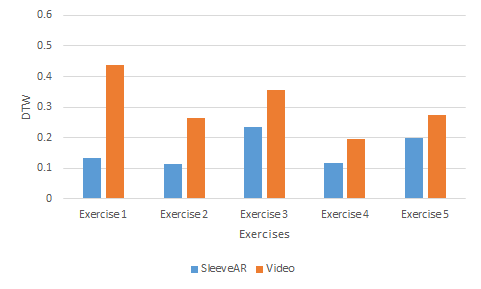
\includegraphics[width=0.8\textwidth]{imgs/results/dtw}
    \end{center}
    \caption{DTW comparison between SleeveAR and observing video.}
    \label{fig:dtw}
\end{figure}

\begin{table}[!t]
\centering
\begin{tabular}{c|c|c|c|c|c|}
\cline{2-6}
\multicolumn{1}{l|}{}                               & \multicolumn{5}{c|}{Exercises}             \\ \cline{2-6} 
                                                    & 1      & 2      & 3      & 4      & 5      \\ \hline
\multicolumn{1}{|c|}{SleeveAR Average DTW}          & 0.114 & 0.148 & 0.326 & 0.129 & 0.380 \\ \hline
\multicolumn{1}{|c|}{Std Dev}                       & 0.090 & 0.148  & 0.201 & 0.059 & 0.276 \\ \hline
\multicolumn{1}{|c|}{Video Observation Average DTW} & 0.439  & 0.263  & 0.355 & 0.195 & 0.273 \\ \hline
\multicolumn{1}{|c|}{Std Dev}                       & 0.165 & 0.092 & 0.170 & 0.066 & 0.0887 \\ \hline
\end{tabular}
\caption{Average DTW from all attempts.}
\label{table:dtwavg}
\end{table}

\begin{figure}[!t]
    \centering
    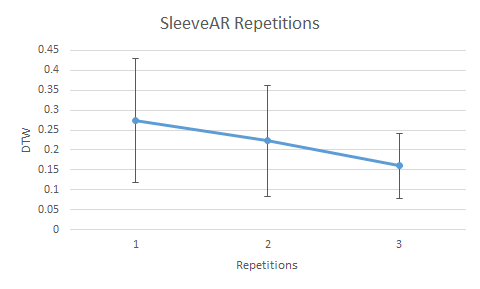
\includegraphics{imgs/results/dtw_repetitions.png}
    \caption{DTW value variation with each repetition using SleeveAR.}
    \label{fig:dtw_repetitions}
\end{figure}

Focusing solely on SleeveAR results, Figure~\ref{fig:dtw_repetitions} presents the average DTW on each of the three trials executed by participants for each exercise. 

These results clearly show an improvement on a patient's performance in just a small number of repetitions. 
Not only the average DTW values become smaller, i.e. closer to the original, with the number of repetitions, but also the standard deviation appears to diminish. 
Indeed, with each repetition, the participant is able to see where he failed the most. Hence,
the system enables improvements on user's next repetition.

We now conduct a hypothesis t-test (test statistic follows a Student's t-distribution) on the slope of the regression line Y = B$_0$ + B$_1$X where B$_0$ is a constant, B$_1$ is the slope (regression coefficient), X is the noise and Y the execution time value.
If there is a significant linear relationship between these two variables, the slope B$_1$ 
will not equal zero. Hence, the hypothesis to evaluate is:
\begin{enumerate}
\item H$_0$: B$_1$ = K. The null hypothesis states that the slope is equal to K (K = 0).
\item H$_a$: B$_1$ $\neq$ K. The alternative hypothesis states that the slope is not equal to 0.
\end{enumerate}
According to Figure~\ref{fig:dtw_repetitions} data, the tscore is 17.4, which results in a p-value of 0.0367.
Thus, the two tailed p-value is lower than the significance level of 0.05, and the null hypothesis is rejected.

In order to evaluate the overall performance from SleeveAR compared to Video observation, a T-Student statistical test was applied to each exercise. 
Our data two data groups for each exercise consisted of their last attempt's DTW value in both alternatives.
Our null hypothesis stated SleeveAR and Video observation average DTW are similar, hence, our goal was to statistically prove SleeveAR enables a lower average DTW. 
This would prove SleeveAR provides a better guidance when replicating exercises.

In Table~\ref{table:ttest} are depicted the calculated p-values for each exercises.
The first four present a p-value lower than \textbf{0.05}. 
By a statistical point of view, we are able to reject the null hypothesis and assume SleeveAR average DTW is in fact lower than using video observation.

As for the last exercise, even though the calculated p-value exceeds the \textbf{0.05} limit, we have detected an outlier that significantly changes this result.
This user generated a SleeveAR DTW value of \textbf{0.85}, more than four times the standard deviation of \textbf{0.187}. 
Therefore, if we chose to remove him from our calculations, a p-value of approximately \textbf{0.004} would be obtained, hence, also rejecting our null hypothesis.


\begin{table}[!b]
\centering
\scalebox{0.8}{
\begin{tabular}{c|c|c|c|c|c|c|c|c|c|c|}
\cline{2-11}
                                              & \multicolumn{2}{c|}{\textbf{Ex. 1}} & \multicolumn{2}{c|}{\textbf{Ex. 2}} & \multicolumn{2}{c|}{\textbf{Ex. 3}} & \multicolumn{2}{c|}{\textbf{Ex. 4}} & \multicolumn{2}{c|}{\textbf{Ex. 5}} \\ \cline{2-11} 
                                              & \textbf{S}    & \textbf{V}    & \textbf{S}    & \textbf{V}    & \textbf{S}    & \textbf{V}    & \textbf{S}    & \textbf{V}    & \textbf{S}    & \textbf{V}    \\ \hline
\multicolumn{1}{|c|}{\textbf{Average DTW}}    & 0,133                & 0,439             & 0,115                & 0,263             & 0,235                & 0,355             & 0,119                & 0,195             & 0,2                  & 0,273             \\ \hline
\multicolumn{1}{|c|}{\textbf{Std. Deviation}} & 0,193                & 0,169             & 0,072                & 0,095             & 0,161                & 0,175             & 0,059                & 0,068             & 0,187                & 0,091             \\ \hline
\multicolumn{1}{|c|}{\textbf{T-Student Test}} & \multicolumn{2}{c|}{0,00002}             & \multicolumn{2}{c|}{0,00001}             & \multicolumn{2}{c|}{0,039}               & \multicolumn{2}{c|}{0,001}               & \multicolumn{2}{c|}{0,145}               \\ \hline
\end{tabular}
}
\caption{T-Student Test for all exercises. SleeveAR(S), Video(V)}
\label{table:ttest}
\end{table}


\section{Validation with Physical Therapist}
\label{sec:pt}

A professional physical therapist, besides the test subjects, also tested the SleeveAR prototype, performing the same exercises as the evaluation ones performed by the test subjects. This expert feedback was afterwards gathered in an interview as a qualitative evaluation of the proposed solution.

First of all, this prototype main vision was to prove we were able to guide subjects through pre-recorded exercises, so the latter were as close as possible of the original exercises. With this in mind, we wanted to evaluate the usefulness of this tool in a regular physical therapy work environment. We also wanted to understand what would be missing to make SleeveAR a more complete tool for a common use along this field of rehabilitation.

We will now present the most significant feedback, stressing both the positive and negative aspects of the proposed solution.


\begin{itemize}
\item \textbf{Missing feedback from one of the three axis}

A fully complete SleeveAR real-time feedback would need to take into account a missing arm movement which is the arm self rotation. Since this prototype focused on guiding the arm through relatively simple movements, we had not previously detected this problem. But, consequently, in the evaluation tests, we realized that it might have helped to take this into account. If a subject has a 90 degree flexion of the arm and maintains the upper arm direction, in case he rotates the upper arm, both the elbow angle and upper arm direction remain the same. Therefore, our prototype assumes it is the same arm position.

\item \textbf{Arm obstructs visibility}

Occasionally, the right arm might obstruct the user's vision, making it difficult to observe the feedback being projected onto the floor. This issue could be solved by projecting all the visual feedback further away from the subject.

\item \textbf{Increase number of tracking points in shoulder area}

In physical therapy, various arm movements also focus on the shoulder area. With this in mind, it would be necessary for our sleeve to contain more tracking points around the shoulder, instead of only having a tracking point for the shoulder, elbow and wrist.

\item \textbf{Potential useful tool for patient reports}

Some physical therapists follow a group of standard arm movements to initially evaluate a patient's condition. With this tool, they could receive full reports with necessary data that otherwise they would have to measure physically. It could be possible to extend SleeveAR to return several additional information about a patient's range of movement after executing a group of exercises. This would allow a physical therapist to have access to patients' information much faster and, possibly, more precisely. 

Additionally, with the possibility of recording movements and later replaying them, SleeveAR could offer a great way of demonstrating the patient, in a visual form, how much he has improved over the course of his rehabilitation, by replaying the historical recordings of his movements.

\item \textbf{A great tool to help a physical therapist when multi-tasking}

While working in a physical therapy gymnasium, therapists often have to look after several patients at the same time. Tools like SleeveAR could help the therapist by lowering the amount of times they have to correct a patient and, therefore, focus on another patient that might need more priority help.


\item \textbf{Provides a great motivation with the feedback received}

The \ac{KP} and \ac{KR} demonstrated in SleeveAR is very satisfactory and could really help in motivating a patient while showing his evolution as he keeps repeating the exercises.

Being able to show how the patient performed by drawing his trajectory over the original exercises helps understanding which parts need improvement. Furthermore, the real-time feedback does a great job at instantaneously showing the patient what to correct on his exercise.

\end{itemize}

\section{Summary}

Overall results show SleeveAR enables its users to perform exercises significantly closer to the prescribed exercises. 
Feedback provided, during and after their performance, allowed for a improvement when repeating their exercises. 
Even if no significant differences were detected on user preference between following SleeveAR or observing video instructions, 
the task performance results clearly show SleeveAR would be a better alternative due to providing user correction in situations they would have none.
Our validation with a physical therapist was vital to enumerate what could still be improved or added to our solution. 
It also confirmed SleeveAR as a possible tool in the rehabilitation field which could facilitate a therapists work in a more advanced phase.